\documentclass[conference]{IEEEtran}
\IEEEoverridecommandlockouts
% The preceding line is only needed to identify funding in the first footnote. If that is unneeded, please comment it out.
\usepackage{cite}
\usepackage{amsmath,amssymb,amsfonts}
\usepackage{algorithmic}
\usepackage{graphicx}
\usepackage{textcomp}
\usepackage{xcolor}

% \usepackage{algpseudocode}

% \usepackage{algorithmic}
% \usepackage{algorithm}

% \usepackage{algorithmicx}
% \usepackage{algorithm}

\usepackage{algorithm}
% \usepackage{algorithmic}
% \usepackage{algpseudocode}

% 中文支持
\usepackage{CJKutf8}

\def\BibTeX{{\rm B\kern-.05em{\sc i\kern-.025em b}\kern-.08em
    T\kern-.1667em\lower.7ex\hbox{E}\kern-.125emX}}
\begin{document}

% 中文支持
% \begin{CJK}{UTF8}{gbsn}

% 文章标题
\title{LaTeX Template for IEEE\\
% 脚注
\thanks{The work is supported by the intelligent software platform development plan 2018 and national college students' innovation and entrepreneurship training program 2020.}
}

\author{\IEEEauthorblockN{1\textsuperscript{st} EternallyAscend}
\IEEEauthorblockA{\textit{College of Software} \\
\textit{GitHub University} \\
Beijing, China \\
ID@github.edu.cn}

\and
\IEEEauthorblockN{2\textsuperscript{nd} Given Name Surname}
\IEEEauthorblockA{\textit{dept. name of organization (of Aff.)} \\
\textit{name of organization (of Aff.)}\\
City, Country \\
email address or ORCID}

% \and
% \IEEEauthorblockN{6\textsuperscript{th} Given Name Surname}
% \IEEEauthorblockA{\textit{dept. name of organization (of Aff.)} \\
% \textit{name of organization (of Aff.)}\\
% City, Country \\
% email address or ORCID}
}

\maketitle

% 摘要
\begin{abstract}
  It's a sample LaTeX template for IEEE. 
\end{abstract}

% 关键词
\begin{IEEEkeywords}
LaTeX, template, IEEE
\end{IEEEkeywords}

% 介绍
\section{Introduction}
It supports Chinese paper if add ``CJKutf8'' package and use font like ``gbsn''.

% 用例
\section{Usage}

% 算法
\subsection{Algorithm}
\begin{algorithm}[htp]
  \caption{\label{SingleColumnAlgorithm}Single Column Algorithm}
  \begin{algorithmic}[1]
    \STATE State.
    \IF    {Situation 1}
    \RETURN{Result 1}
    \ENDIF
    \IF    {Situation 2}
    \STATE State.
    \IF    {Situation 3}
    \STATE \textbf{Goto} Step 2. % \emph{Request}.
    \ENDIF
    \RETURN{Result 2}
    \ENDIF
  \end{algorithmic}
\end{algorithm}

\begin{algorithm*}[htp]
  \caption{\label{DoubleColumnAlgorithm}Double Column Algorithm}
  \begin{algorithmic}[1]
    \REQUIRE User Send Access Request of Target A via Client and Start Listening.
    \WHILE {No Privileges}
    \STATE Query Superior Organization and Check Status.
    \IF    {Superior Organization Not Exists or Status is False}
    \RETURN{No Privileges}
    \ENDIF
    \ENDWHILE
    \RETURN{Encrypted Data}
  \end{algorithmic}
\end{algorithm*}

% 图片
\subsection{Figure}
\begin{figure}[htbp]
  \centerline{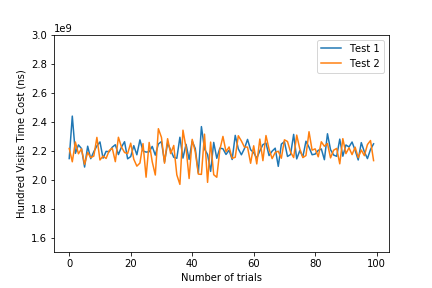
\includegraphics[width=8cm]{figures/Query_Label.png}}
  \caption{Algorithm \ref{SingleColumnAlgorithm} via Single Column Figure\label{SingleColumnFigure}}
\end{figure}

\begin{figure*}[htbp]
  \centering
  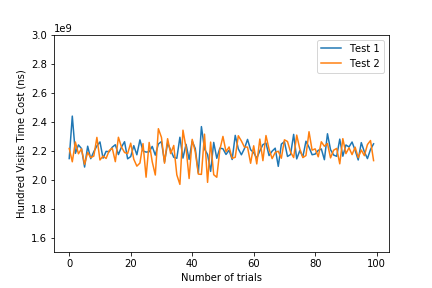
\includegraphics[width=10cm]{figures/Query_Label.png}
  \caption{Double Column Figure\label{DoubleColumnFigure}}
\end{figure*}

% 表格
\subsection{Table}
\begin{table}[http]
  \centering
  \caption{Single Column Table}
  \label{SingleColumnTable}
  \begin{tabular}{c|cc}
    \hline\hline
    A & B & C \\
    \hline
    D & E & F \\
    G & H & I \\
    Other & ... & ... \\
    \hline\hline
  \end{tabular}
\end{table}

\begin{table*}[http]
  \renewcommand{\arraystretch}{2}
  \centering
  \caption{Double Column Table}
  \label{DoubleColumnTable}
  \begin{tabular}{ccccccc}
    \hline \hline
    Organization & Root & Add & Control & Urgency Access & Write & Read \\
    \hline
    Root & 1    & 1   & 1       & 0              & 0     & 0    \\
    Administrator&0&1 & 1       & 0              & 0     & 0    \\
    Other & ... & ... & ...     & ...            & ...   & ...  \\
    \hline \hline
  \end{tabular}
\end{table*}

% 参考文献和引用
\subsection{Cite and Ref}
In paper \cite{eternallyascend2023latex4ieee}, the Algorithm \ref{DoubleColumnAlgorithm}, Figure \ref{DoubleColumnFigure} and Table \ref{DoubleColumnTable} are different to the Algorithm \ref{SingleColumnAlgorithm}, Figure \ref{SingleColumnFigure} and Table \ref{SingleColumnTable}

% 总结
\section{Conclusion}
The result is that you can use this template not only for IEEE paper but also other reports.

% 未来工作
\section{Future Work}
Here is nothing in the TODO list now.

% Reference

\bibliographystyle{abbrv}
\bibliography{reference.bib}

% \begin{thebibliography}{00}
%     \bibitem{bitcoinNankamoto}
%     Satoshi Nakamoto.
%     \newblock Bitcoin: A peer-to-peer electronic cash system.
%     \newblock {\em Bitcoin. --URL: https://bitcoin.org/bitcoin.pdf}, 4, 2008.
% \end{thebibliography}

% 中文支持
% \end{CJK}

\end{document}
